\chapter{Implementation Approach}
\label{chap:implementation}
\lhead{\emph{Implementation Approach}}
\usepackage{graphicsx}

Identifying the best technologies to utilise in order to design the drowsiness detection system enables the objectives of the project to be met.  Understanding how each technology would fit into the architecture and function with one another meant researching various alternative approaches. In order for me to fully design and implement this project successfully I will need to carefully layout out a path to successfully build my project from the ground up while trying to minimize all the issues that I will encounter on the way.
Now I must specify my initial first understanding of what the system is required to do, I will look at drafting a first outline of a software system to meet the requirements that must be met in order of fulfilling the task of fully. It is not the goal of this outline to prescribe the implementation of every detail of the system, but rather to gain an overall idea of the technologies, subsystems and components involved; their relationship to each other; and the role they play in the system. It also presents us with another chance to uncover complex, badly understood, or other potentially problematic areas of the system—crucial knowledge when it comes to estimating the work load (cost) during the planning of the project implementation.
The type of system this project is a Embedded hardware based system and the architecture, what I will be detailing moving forward for this system will detail everything that this system will consist of; I will be discussing the languages used for the project itself, languages will vary as there will be other components involved in this project itself , such as a database query language, beyond this I will discuss the core libraries that this project will require, external technologies that could be used to help with facial detection and recognition when drowsiness has been detected. Along with this I will detail the core methods that will be used in this project, machine learning techniques such as cascade classifiers will be used and how this will be implemented in within the system and how it occupies, eye detection techniques will be specified and will be placed accordingly within the architecture implementation.
 ]
\section{Architecture} \label{sec:Arch}
\begin{itemize}
    \item Technologies involved ( Python, opencv, numpy, Firebase, ). 
    \item The hardware needed to develop the project (5 mega pixel camera, Speakers)
\end{itemize}
\subsection{Design Model}
The architecture of this project will most likely be modeled with a blackboard design model, choosing this design model suits the type of system that I will design going forward the reason for this is because the blackboard design model is a model design suited for systems where their is a heavy emphasis on the data input that is inputted heavily and continuously into the
system and the system having to make some decisions to solve the problem at hand, this type of of design pattern is used typical for speech recognition as it is most often cited within system involving speech recognition although a design pattern mostly used in speech recognition. The blackboard model is perfect for any system where their is an emphasis on the system performing any type of recognition such as within the drowsiness detection system where their is a great emphasis on facial recognition. The Blackboard model's Unified Modeling Language dictates that this framework mostly consist of the blackboard, the controller and one or more knowledge sources, the blackboard will receive the input from the camera by a continuous stream where it will then inform the controller in which the controller will enroll a knowledge source whereby the function of the knowledge source is to perform is to process the data that is obtained by the blackboard object. The knowledge source would have a thread that would process the blackboard object that it has retrieved, once this object has been processed the blackboard would be updated with a partial solution blackboard object that would then be processed and the controller would finally be notified setting the flag to be true. The blackboard, controller and the knowledge source will all have an abstract class, to detail the process that would generally occur and how the flow would be like within this framework I must verify how the stream of data will be dealt with initially by the blackboard class, when the blackboard class receives a new blackboard-object the blackboard class notifies the controller class when the controller is updated with a new blackboard-object, it queries the knowledge-source with the blackboard-object so that it can see who would like too handle the task that the blackboard-object brings with it, once a knowledge-source has accepted the task it would then spawn a new thread, the blackboard controller class must then wait for the a response from the knowledge-source for a reply the tasks that it has chosen to take up from the blackboard class itself, once the task is complete and the controller receives a response with the initial blackboard-object and accompanied by the is-ready flag set to true. The controller then quickly calls the execOutcome(Blackboard's-Object boo) in-order to finish off the the process.

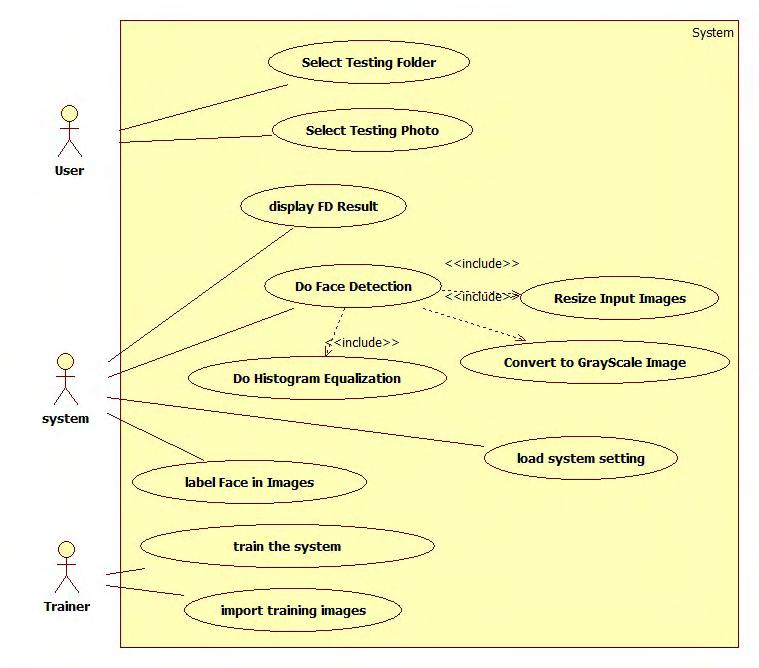
\includegraphics[width=0.9\textwidth]{Figures/UMLDrowsinessDetection.jpg}

This model is very straight forward and doesn't require to many classes like other other design frameworks for example the layered pattern which would have a downwards case layout when looked at through the unified modeling language diagram, with this type of model there isn't any loop back that can inform previous classes if an object received by the current class has been detected to have an issue which can disrupt the accuracy of the program entirely, as the data being received can be incorrect for example if camera being used doesn't identify the face and starts targeting other landmarks within the image, how would a layered model overcome this. The blackboard model will reduce the complexity of the program entirely so that a cleaner system can designed can be built.
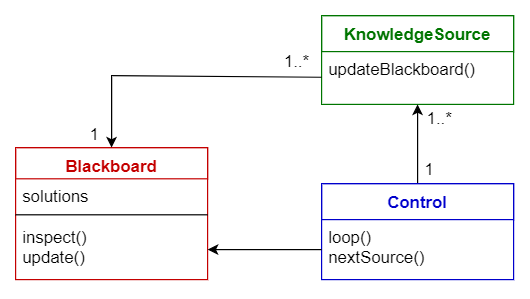
\includegraphics[width=0.8\textwidth]{Figures/Blackboard.png}
\subsection{Technologies}
A number of technologies that will be used along with this model will consist mainly of libraries and a possible external open source  technology that will be used for facial recognition. The main library that will be used will be the OpenCV and will be used for the machine learning and computer vision features that the library consists of. 
The OpenCV supports many interfaces but the interface that will be used within this system will be the python language. OpenCV has as much as 500 algorithm's that aids with real-time vision applications. The methods provided by the OpenCV such as VideoCapture() method will be used within the drowsiness detection system to access the camera and to set the capture Object as cap.read() this method will perform the process of reading each frame of the video being recorded by the camera and to store each individual frame as an image that would then be stored in a frame variable that will be created. Haar cascade classifiers may be used from this point on, the OpenCV library has methods dedicated to the use of this algorithm CascadeClassifier(‘ path to our Haar cascade XML file’) this is a process within the system that will be accompanied by a detectMultiScale(gray) this method will most likely be used to as the image will be converted in grey scale. OpenCV has a algorithm for object detection that will only take input in grey scale so when using the detectMultiScale(gray) it processes the new gray scale image that was converted from the real time image that was taken in by the camera, the detectMultiScale(gray) method is in place so that it can return an array of detection which consist of coordinates that can be plotted on an x and y axis this is all done so that the system can detect the the faces in an image and create a region of interests, this region of interest will be the eyes. 

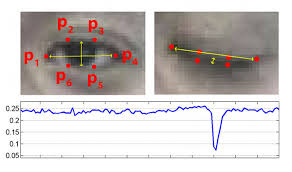
\includegraphics[width=0.8\textwidth]{Figures/eyeDetection.jpg}

The same Process will be done yet again but this time both eyes will be stored within the d method that detectMultiScale(gray) method that is within the OpenCV library. The is done so that images can be fed to the cascade classifier so that it can perform an analysis of the eye determining if the eye is open or closed. The Haar cascade classifier will run some test depending on the result of the images that it has processed internally within the algorithm and from here it can provide a score to determine if the the individual is drowsy or is not. The Drowsiness calculation is determined by a score, this score is calculated by timing how long a person has closed their eyes for. Their will be a threshold in place and the user will be alerted. 
\subsection{Database}
A back end database will be in place such as Firebase so that an administrator monitoring the drivers who are feeling drowsy can then assess the state in which the drivers are performing. A method will be used to perform continuous serialization, this is a process of converting an object into a stream of bytes so that it can be stored in a file, database or memory. Its main purpose is to save the state of the object out putted in final operation of the Drowsiness detection system so as to keep track of which current drivers are feeling drowsy and to send a personal alert to the driver to inform the driver that he is exhibiting too many instances of drowsiness and that he must take a break or otherwise he might be in danger on the road, this database will have the drivers details such as first and last name accompanied by his driver id number. Firebase stores data in real time in a JavaScript Object Notation format, Firebase database is able to perform certain functionalities such as sending an email or sending a one time code to a phone number that has been provided to the database. A simple PIP installation is required to set up Firebase database within the Drowsiness detection system, this is all that will be required so that a Firebase database implemented into the system.

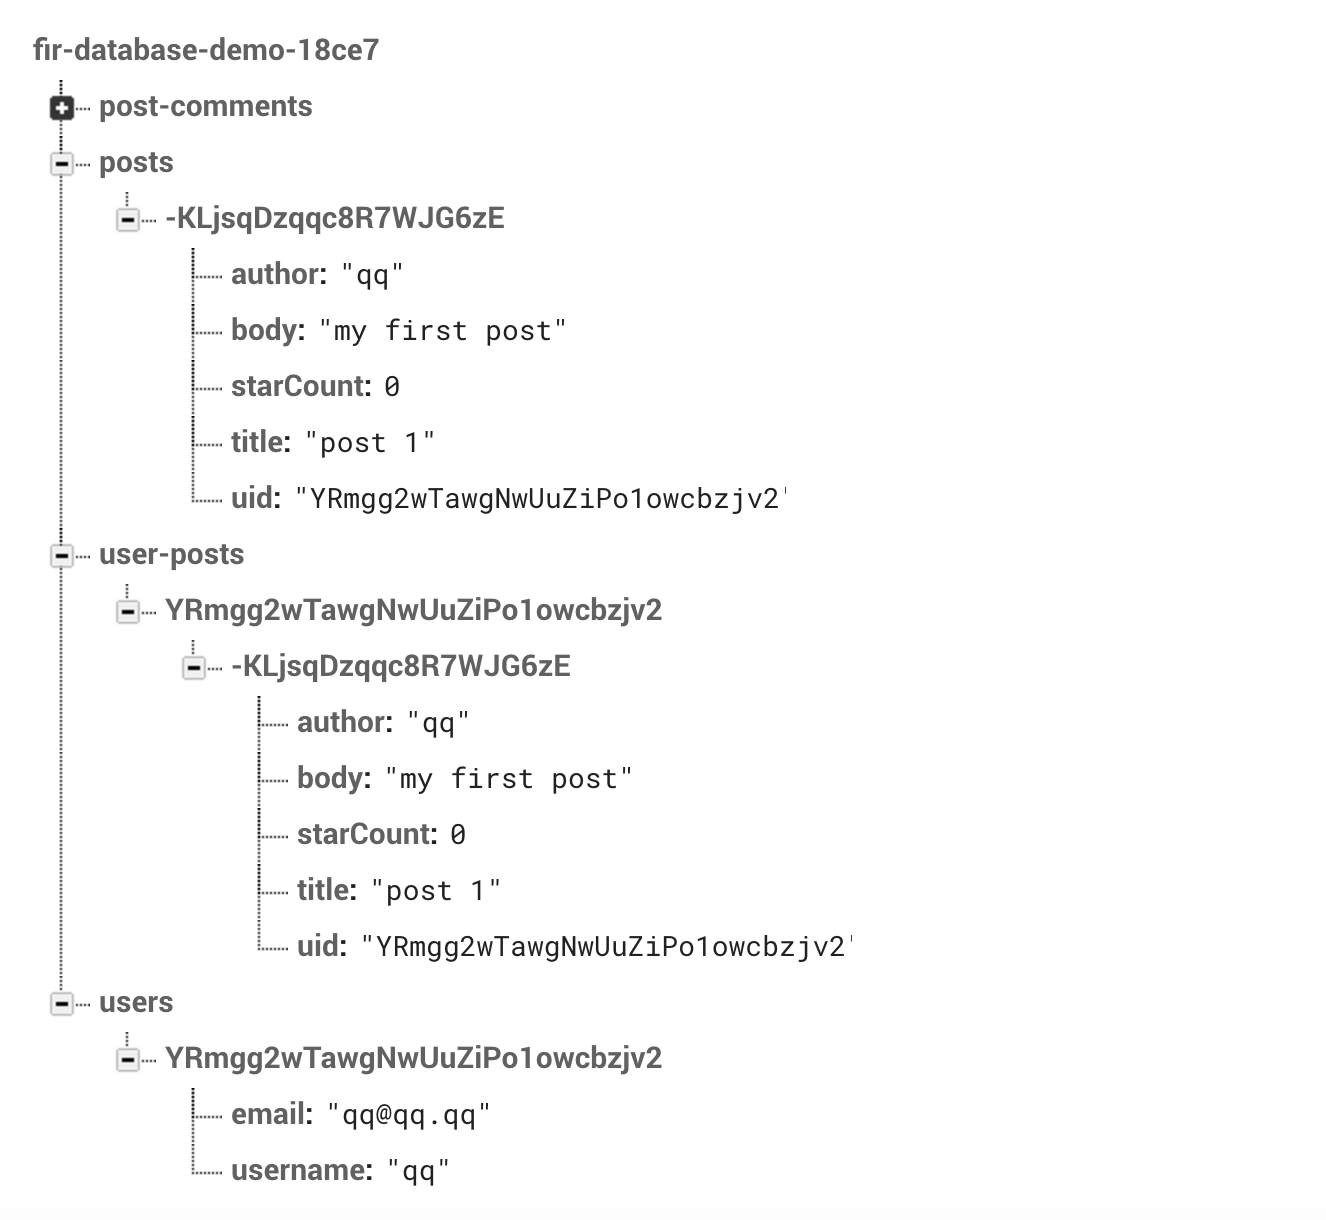
\includegraphics[width=0.8\textwidth]{Figures/Firebase.png}

\subsection{Framework}
Through this project the Python language will be used as it is commonly know as a general purpose language and accompanied by many libraries and tools that are designed for the python language most of the libraries have been detailed above that I will be using in this system.  Python is an excellent language and is the perfect choice for implementing within the architecture of this system. Python is well know for its  backend web development, data analysis, artificial intelligence, and scientific computing. When designing this system their will be a huge emphasis on artificial intelligence, with algorithms such as cascade classifiers that have to be implemented in the system these algorithms can be found inside The OpenCV library but implementing this library in python is very easy and only requires a quick import. Importing libraries into python is much more straight forward. The final design will have most likely have 4 or 5 python scripts that will communicate which each other, their will be a script Dedicated to reading the input from the camera and converting each frame to a grey scale copy which will then be accompanied by a script that will  implement Haar Cascade classifiers algorithm on the frames received of the face and the eyes, their will be a script that will then perform a threshold test that will determine if the the users is exhibiting drowsiness within the frame and then will sound an alarm if present and the final script will be a script that will perform backend database operation with Firebase database uploading the outcomes of each instance when a detection has successfully been detected and which driver triggered this. The integrated development environment that will be used to develop this system will be Pycharm as it is free has cross platform functionality and can easily integrate any backend database I require. 
This is everything I currently believe will be required by the Drowsiness detection system in term of architecture going forward 


\section{Risk Assessment }
\begin{table}[h]
\centering
\scriptsize
\caption{Initial risk matrix}
\begin{tabular}{|p{2cm}|p{2cm}|p{2cm}| p{2cm} |p{2cm}| p{2cm}|}
\hline \bf Frequency/ Consequence & \bf 1-Rare & \bf 2-Remote & \bf 3-Occasional & \bf 4-Probable & \bf 5-Frequent\\ [10pt]

\hline \bf 4-Fatal & \cellcolor{yellow!50} & \cellcolor{red!50} & \cellcolor{red!50} & \cellcolor{red!50} &\cellcolor{red!50} \\ [10pt]

\hline \bf 3-Critical &\cellcolor{green!50} & \cellcolor{yellow!50} & \cellcolor{yellow!50} & \cellcolor{red!50} &\cellcolor{red!50} \\ [10pt]

\hline \bf 2-Major & \cellcolor{green!50} & \cellcolor{green!50} & \cellcolor{yellow!50} &\cellcolor{yellow!50} &\cellcolor{red!50} \\ [10pt]

\hline \bf 1-Minor & \cellcolor{green!50} & \cellcolor{green!50} & \cellcolor{green!50} &\cellcolor{yellow!50} &\cellcolor{yellow!50} \\ [10pt]
\hline
\end{tabular} \\
\label{tab:ProjRisks}
\end{table}
As with Any system their can be many risks when first undergoing development of a system, so to for-tell if issues may arise within the drowsiness detection system we must carefully analyse all the the tasks currently understood that is required to be implemented so that a successful system can be deployed. Even though I have ensured completely that this project is carefully planned out, there is still a possibility of it running into trouble, their is always a possibility  and over the years even regardless of how I have mapped out my project work I have encountered risks that have halted my progress to completing a project with a complete and fully functioning requirements.   A  risk  in  simple way to understand  is  any  uncertain  event  or  condition  that  may  effect a developers project that has been undertaken.  However, any risk may be a scary occurrence to any developer as the developer is entering into unfamiliar territory, but not all risks are completely bad and encountering issues within a developers project can benefit the the developer in a multitude of ways for example,  one can find a  much better, easier and viable way to  implement  a certain  feature into their project,  which  can  benefit the  project and the developer.   There  is  no  guarantee that a project will be successful, so developers must be ready to handle any risk that occurs small or large. Developers learn from the risk that they faced on each project that they have taken up and have grown as engineers, becoming much more viable to their employers and the companies they work in. 
This section will detail all the possible risk that I may occur when I start the implementation face of this project.

\subsection{Hardware or software failure}
This project will be running on Lenova yoga 520 laptop with a hardware specification set with Central processing unit consisting of a Intel Pentium 4415U 140,  Graphical processing unit consisting of Intel High Definition Graphics 610 236 with a Display that is  14.0" inches, the
Lenova yoga 520 laptop has a built in camera that will be used for image processing has an internal mic and 4 speakers that will be used for sounding the alarm in the event of a drowsiness detection threshold being achieved.
\subsection{Hardware failure 1.1}
A risk that can occur in this project is that the camera or speakers that my laptop possesses fails to work when I am developing my project this issue can occur at any point during my implementation phase of this system, this is a risk that would stop my project from fulfilling  core functionality requirements within the system. This isn't the only issue that may occur in relation to hardware if a complete system failure occurs, I may lose implementation's progress and depending on which Stage I am at all my progress may be lost, progress may be lost. This may not be a common risk but I have encountered complete system failure during collage semester and project cycles. This type of risk can easily be avoided and one of the best data protections tools on the internet is to upload each bit of progress onto GitHub having a private repository in which only I have access to and where I can push each new commit, this allows for my any work done in during the implementation phase of this system to be phase and in the event of a system failure any other computer can be used to login and access my my repository and work can be continued on the system just from where I have left it before the system hardware failure. This is also the case if the Hardware failure is component based, another laptop can be used with components that are working.

\subsection{Software failure 2.1}
Another risk that may occur during the development of this is that a software failure may occur that can completely stop all my progress when it comes to developing this system, if when developing this system certain libraries that I plan on using for this project are not compatible with the hardware of my computer this can cause a major risk in the implementation phase of the system, This can be a major issue if I encounter this during development as I could have to re-decide how I will re-implement my project and can hinder progress cutting time off of the remaining time that I have left when I have to fully develop my project. Luckily when when doing my research of the technologies that I will use during for this system, everything from the languages to the libraries used are well supported and commonly used in modern applications to perform ta multitude of task so this risk is severely minimised.  If this case does happen during the implementation phase the risk wont be too great when it comes to re implementing the projects as there has been extensive research undertaken by major car organisations and fellow developers and researchers, and a multitude of different implementation techniques have been undertaken so the re-assessing time will be very minimal.
\subsection{Requirements 4.5}
Given that the development of this system is self managed by myself there is a risk of the requirements being in-adequately defined and undertaken by myself during the implementation phase of my project. During the implementation phase I may discover a requirement change or a task being unnecessary during implementation but if this happens it is possible to work around this because the core value requirement this system possesses are very difficulty to change and the likelihood of a requirement change showing up will be very rare.Their may be a decision on my end to change something about the system, and this may lack the full understanding of how how big of an impact it will have on the system.  To prevent this, good and thorough communication must be done with my supervisor and must be constant so that if any change of plan for the implementation phase needs to be designed my supervisors feedback will help me visualise this impact and if it is a good decision or isn't a good decision .
\section{Methodology}
As this is a system that will be managed by myself during the implementation phase, it is important to keep a concise list of goals that must be undertaken,  Common software methodologies such as Agile and waterfall methods during software development projects  for self-managed  projects are not typically undertaken as most  of  the  time they are in place for  team-based projects such as the the car pooling application that I have undertaken in year 3 semester 1..  The waterfall model is still used in large parts of the industries, but in many instances within the industry, it is used in combination with other methodologies, meaning its used in parallel with another very popular and commonly used model, such as Agile.  The model allows for easy a much easier testing and analysis but does not allow updating and re-implementation during the testing phase. The Agile development methodology used within the industry is a very popular approach across majority of the tech and software industries.  It is an approach that allows for adaptation and that responds to changes that are liked upon and are favorable but there are chances of deviation that can occur and this causes outcomes that are not clear. The scrum programming methodology is the methodology that I will be implementing during the implementation phase of my project with Scrum, software is developed using an iterative approach in which the team is front and center, disciplined workers on smaller teams might find the most success with this method, as it requires self-organization and self-management.

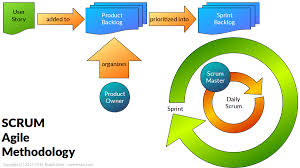
\includegraphics[width=0.8\textwidth]{Figures/Methodologies.jpg}

Team members would usually break down the end goals of a project into smaller goals so that at the beginning  of a projects they can work through them using iterations that are a  fixed length or by industry  what understood in the industry as a process called sprints to help build software and showcase it often to each other in the team, sprints usually only last  up to two weeks. Meetings play an important role in  in the Scrum approach ,and because of how the implementation phase will consist of supervisor meeting this is a very valid methodology for me to use. each sprint cycle will consist of daily planned  meetings where demos will take place to follow progress and gather feedback. Due to this, the incremental method promotes quick changes during the development cycle and adds excellent value to this complex system implementation that I will undergo. Scrum incorporates the structure and discipline of more traditional software development methodologies with the flexibility and iterative practices of modern Agile and due to this it makes scrum a very viable methodology for myself to use during the implementation phase of the drowsiness detection system.

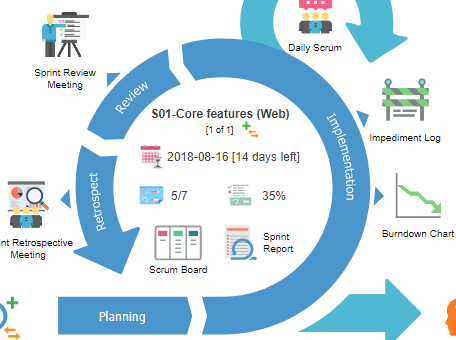
\includegraphics[width=0.8\textwidth]{Figures/Scrumchart.png}

There may be a few things that are new and need to be studied thoroughly in order to fully complete this project.  The first thing I like to do when I have encountered a new technology that I need to learn  as something new is to primarily focusing on the important sections and fundamental concepts that the new material consists of.  When it comes down to whatever it is that needs to be learned in order to complete this project. There are excellent sites that have tutorial on how to fully understand the new material that I have encountered, another important requirement of learning something new is planning and the quality of time that is allocated for it .

A good Implementation Approach of fundamentals discussed earlier when it comes to learning, is to best to choose a  environment very well suited to learning something new for example a learning environment with  no distraction. I quite room at home should be sufficient  just for learning or collage or local library would be sufficient enough when it comes to finding a suitable environment also.  It is  very important to gather a wide range of excellent resources of material that one will need to learn and to gather  so a very good understanding of the new material one must understand can be achieved. 

When trying to fulfil the Background chapter during this phase, an experienced developer will need to understand what area of Computer science the project resides within.  This requires extensive time and research as with each discipline there are a multitude of areas that must be understood, Computer Science is no different.  Firstly and  most importantly  one must  research of similar projects relating to the project at hand.  This gives a very good vision of what others have done  with projects at are within the same area that the project being researched resided in.  Having a good formulate understanding cannot be advised of one ́s project is without a doubt highly recommended, due to ones needs within the project having the ability to distinguish the differences between projects that already exist and their own project.
\section{Implementation Plan Schedule}
For the schedule I have planned during the implementation phase what I must do in the  time given to me for this project,  is to use the  duration  of  the second semester, and the time allowed to me wisely. The approach taken to make sure this project is completed is an iterative and incremental this has already been dictated by the methodologies section where I have discussed this earlier. Each of my increments we done  in equal time duration from each other.  Below I have listed all the tasks that I plan to do from the beginning to the end this should Provide the right type idea how my project implementation will be progressed from the beginning cycle until the end

\includegraphics[width=0.5\textwidth]{Figures/flowchart.png}

\begin{itemize}
\item Task 1 - Install all the required software and technologies that my system will require for example PyCharm, PyGaze, OpenCV and install Firebase into working environment.
\item Task 2 - Configure all the technologies so that my working environment has all the technologies present and running the correct version. 
\item Task 3 - Download the blackboard design model script and Begin implementing OpenCV Methods and class can work start making use of the camera components on my computer. 
\item Task 4 - Perform frame capturing functionality so to convert these frames into grey scale so that the Haar cascade classifier algorithm can start to do facial recognition 
\item Task 5 -Begin developing Haar cascade classifiers algorithm in order to use the algorithm to identify I users face.
\item Task 6 - Once developed train the algorithm start identifying a users face in each frame that is captured. 
\item Task 7 - Once the Haar cascade classifier has been trained to detect faces from each frame that is extracted of the users face then begin to train the Haar cascade classifier algorithm to detect the users eyes.  
\item Task 8 - Finally by using the Perclos algorithm to calculate the eye open to eye close ratio an score can be retrieved so that an threshold can be configured in order to detect if a user is feeling sleepy. 
\item Task 9 - Configure Alarm functionality with the speaker components on the on the computer so that when the threshold has been exhibited by the driver then the alarm will be sounded.
\item Task 10 - Begin database implementation to the system and this will be one of the final tasks to be done.
\item Task 11 -Set up JSON script inside the FIREBASE database with parameter consisting of the users details and drowsiness ratio 
\item Task 12 - Configure the serialization of data from the system to the backend database 
\item Task 13 - When drowsiness occurs with the driver then the admin monitoring the Database will be informed
\item Task 14 - Final test of the the system will be done to ensure the requirements have been met.
\item Task 15 - Provide comments and explanations of what the code does, tidy up the code in area need tidying up. 
\end{itemize}

\section{Evaluation}
When evaluating  all the goals their will undoubtedly be objectives that are achieved  quickly, while others will need some considerable  planning.  When planning is done for these tasks smaller goals can targeted allowing for the system to be developed more efficiently. These goals must  be maintained by a time bracket, this is very important in the system, Time brackets will allow the developers to measure the progress of each goal. A common approach in a project task is to simplify the task and ensure that it provides value.My final evaluation can help me learn what has been a success and what was  not  a success within this project.By understanding what this project is trying to achieve, this understanding is the core factor in understanding understanding the core evaluative measure to having a successful completion is this system come the end of next month .  To do this one I identify the project ́s objectives and they are to have a Drowsy detection system, a system that will detect if a driver is drowsy and this is done if the system can successfully detect if the user of the systems eyes are closed and this is done only when the systems algorithms and libraries are can fully extract this data from the camera on the computer. This is how i will be forming my evaluation of a successful system design design and implementation.


\section{Prototype}
Although no implementation has been done yet I carried out a few test with some of the libraries using OpenCV.

The first Test I carried out was a simple library test to see if OpenCV worked. I wrote a small script.

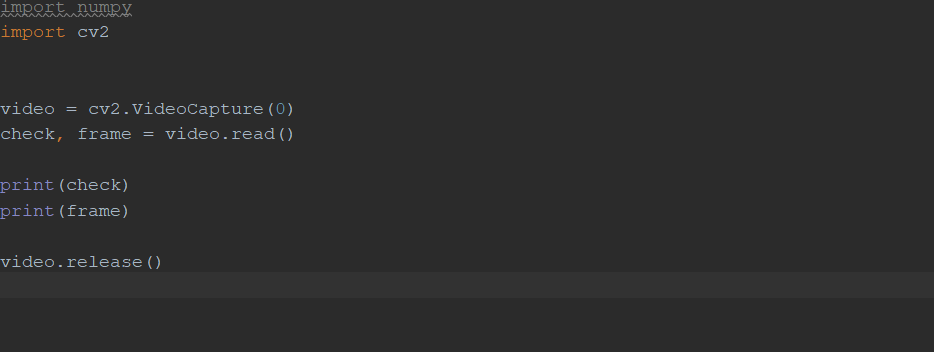
\includegraphics[width=0.8\textwidth]{Figures/Pythonscript.png}

This was the first Python script that I ran.  I ran this script so that I can observe what the terminal would output and a received what I expected from the terminal, which was matrices with zeros residing inside them. The reason They are displaying zero is because  the camera isn't active and isn't picking up any frames.

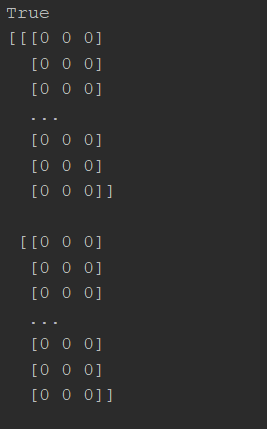
\includegraphics[width=0.8\textwidth]{Figures/terminalPythonScript.png}

This above image will show you what I the output received when I ran the script, you will see multiple matrices with zeros residing within them as i outlined before. 

I then updated my script so that I can have the camera show up on my screen although the camera is turned off by default in my setting this script shows that the OpenCV library methods are communicating with with my computer and very efficiently also.

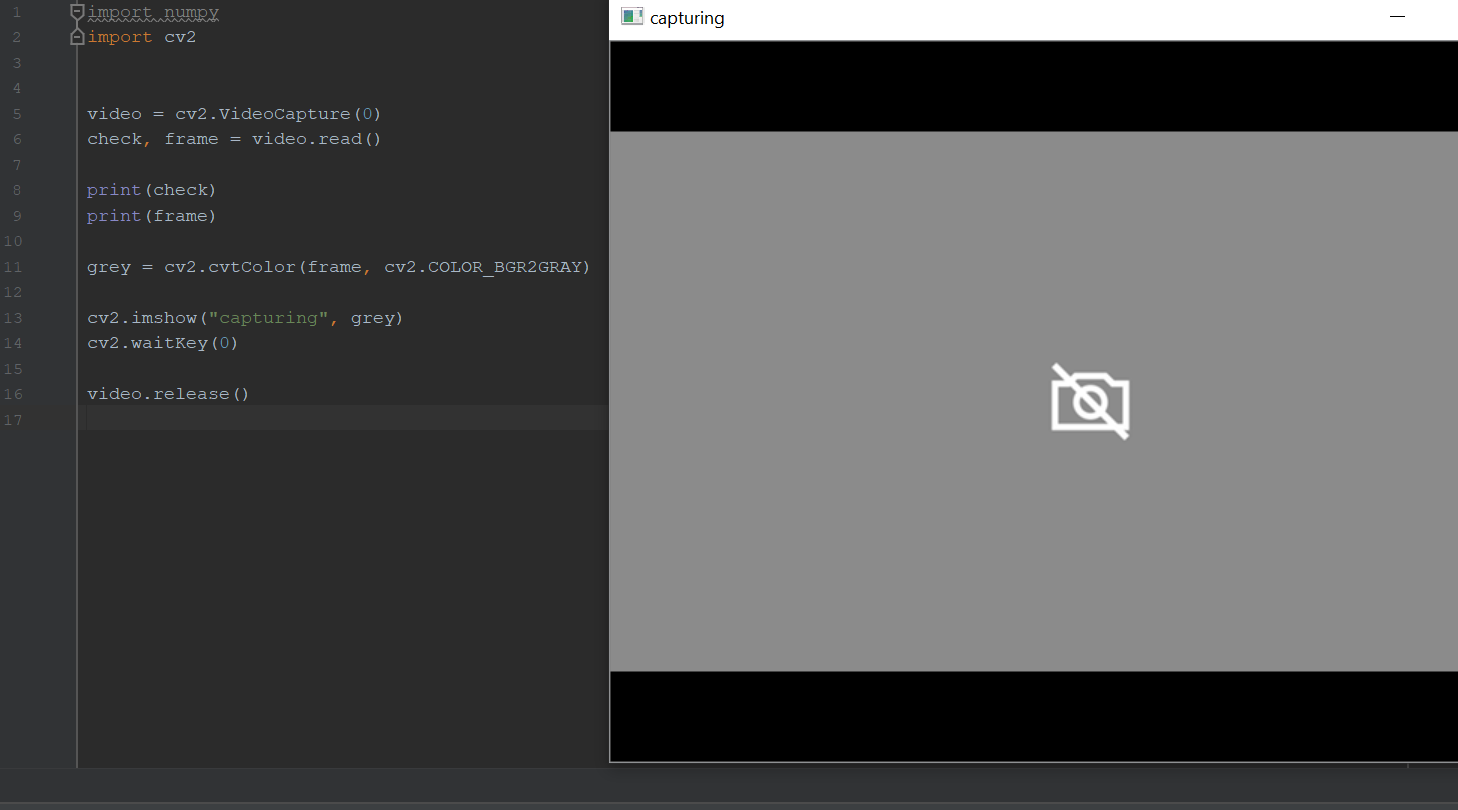
\includegraphics[width=0.8\textwidth]{Figures/Pythonscriptwithcamera.png}

AS you can see I have added a few more methods and have used a method to convert each new frame to grey scale this cant be seen as their is new picture but the functionality is within the code.




